\documentclass[DIV=24]{scrartcl}
\usepackage{tikz}
\usetikzlibrary{positioning}
\usetikzlibrary{shapes}
\usetikzlibrary{arrows}
\usepackage{fontspec}

\usepackage{listings}
\usepackage{graphicx}

\definecolor{mygreen}{rgb}{0,0.6,0}
\definecolor{mygray}{rgb}{0.47,0.47,0.33}
\definecolor{myorange}{rgb}{0.8,0.4,0}
\definecolor{mywhite}{rgb}{0.98,0.98,0.98}
\definecolor{myblue}{rgb}{0.01,0.61,0.98}

\newcommand*{\FormatDigit}[1]{\ttfamily\textcolor{mygreen}{#1}}
%% http://tex.stackexchange.com/questions/32174/listings-package-how-can-i-format-all-numbers
\lstdefinestyle{FormattedNumber}{%
	literate=*{0}{{\FormatDigit{0}}}{1}%
	{1}{{\FormatDigit{1}}}{1}%
	{2}{{\FormatDigit{2}}}{1}%
	{3}{{\FormatDigit{3}}}{1}%
	{4}{{\FormatDigit{4}}}{1}%
	{5}{{\FormatDigit{5}}}{1}%
	{6}{{\FormatDigit{6}}}{1}%
	{7}{{\FormatDigit{7}}}{1}%
	{8}{{\FormatDigit{8}}}{1}%
	{9}{{\FormatDigit{9}}}{1}%
	{.0}{{\FormatDigit{.0}}}{2}% Following is to ensure that only periods
	{.1}{{\FormatDigit{.1}}}{2}% followed by a digit are changed.
	{.2}{{\FormatDigit{.2}}}{2}%
	{.3}{{\FormatDigit{.3}}}{2}%
	{.4}{{\FormatDigit{.4}}}{2}%
	{.5}{{\FormatDigit{.5}}}{2}%
	{.6}{{\FormatDigit{.6}}}{2}%
	{.7}{{\FormatDigit{.7}}}{2}%
	{.8}{{\FormatDigit{.8}}}{2}%
	{.9}{{\FormatDigit{.9}}}{2}%
	%{,}{{\FormatDigit{,}}{1}% depends if you want the "," in color
	{\ }{{ }}{1}% handle the space
	,%
}


\lstset{%
	backgroundcolor=\color{mywhite},   
	basicstyle=\footnotesize,       
	breakatwhitespace=false,         
	breaklines=true,                 
	captionpos=b,                   
	commentstyle=\color{red},    
	deletekeywords={...},           
	escapeinside={\%*}{*)},          
	extendedchars=true,              
	frame=shadowbox,                    
	keepspaces=true,                 
	keywordstyle=\color{myorange},       
	language=Octave,                
	morekeywords={*,...},            
	numbers=left,                    
	numbersep=5pt,                   
	numberstyle=\tiny\color{mygray}, 
	rulecolor=\color{black},         
	%rulesepcolor=\color{myblue},
	showspaces=false,                
	showstringspaces=false,          
	showtabs=false,                  
	stepnumber=2,                    
	stringstyle=\color{myorange},    
	tabsize=2,                       
	title=\lstname,
	emphstyle=\bfseries\color{blue},%  style for emph={} 
}    

%% language specific settings:
\lstdefinestyle{Arduino}{%
	%basicstyle=\ttfamily,
	style=FormattedNumber,
	keywords={void,digitalWrite,pinMode,const,int,bool,unsigned,long,delay,if,else,switch,case,millis()},%                 define keywords
	morecomment=[l]{//},%             treat // as comments
	morecomment=[s]{/*}{*/},%         define /* ... */ comments
	emph={HIGH, OUTPUT, LOW,false,true},%        keywords to emphasize
}



\newcommand{\oreProgrammate}{\color{red}{oreProgrammate}}
\newcommand{\tempoAspegnimento}{\color{blue}{tempoAspegne}}
\newcommand{\conteggioAttivo}{\color{green!60!black}{conteggioAttivo}}

\date{\today}

\begin{document}
    \setmainfont{DejaVu Sans Mono}
    %\maketitle
    \tableofcontents
    \begin{abstract}
    	Modifiche versione 4:
    	\begin{itemize}
    		\item correzione errori nella base dei tempi (Pa=Qa-Xa e Pb=Qb-Xb)
    		\item impostate ore 2,4,6,8
    		\item spegnimento del led sulla porta 13 dopo un lampeggio iniziale quando si collega il circuito
    	\end{itemize}
    	\bigskip
        Il circuito è un timer programmabile per l'accensione e lo spegnimento automatico della pala del ventilatore. 
        \begin{itemize}
        \item Il timer si attiva premendo il pulsante. 
        \item L'indicazione del tempo programmato è visualizzata da quattro LED luminosi che si accendono progressivamente ad ogni pressione del pulsante.
        \item Alla quarta attivazione il tempo impostato riparte da zero.        
        \item Una pressione prolungata del pulsante permette di spegnere il timer se risulta già acceso. Se  spento, la stessa prolungata accensione ne determina l'attivazione di un tempo predefinito pari a tre LED accesi.
        \end{itemize}
    \end{abstract}
    \section{Schemi a blocchi}    
    \subsection{loop}
    \begin{center}
        {\scriptsize
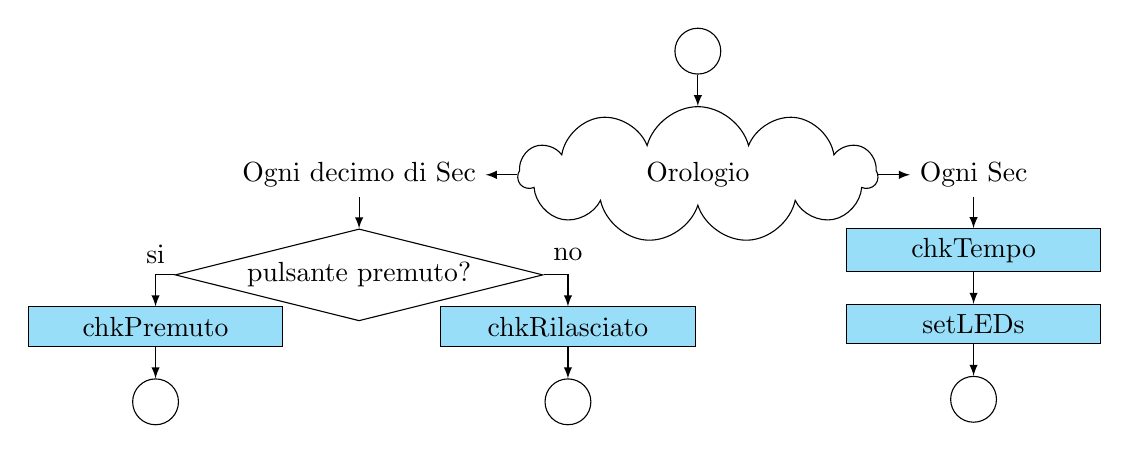
\begin{tikzpicture}[align=center,minimum height=5mm,node distance=4mm,
affermativo/.style={anchor=south east},
negativo/.style={anchor=south west},
testo/.style={draw,text width=3cm,anchor=north},
testoC/.style={text width=3.5cm,anchor=center},
condiz/.style={draw,diamond,aspect=4,text width=3.5cm},
cerchio/.style={draw,circle,text width=0.7cm}
]
%--
\node[cerchio,text width=3mm,](a){};
\node [testo,cloud,cloud puffs=11,draw,cloud ignores aspect, fill=white,below=of a] (b)  {Orologio};
\draw [-latex] (a) -- (b);
%--
\node[left = of b](decimo){Ogni decimo di Sec};	
\draw [-latex] (b) -- (decimo);	
\node[right = of b](sec){Ogni Sec};	
\draw [-latex] (b) -- (sec);	
%--
\node[condiz,below = of decimo](a){}; \node[testoC] at (a.center){pulsante premuto?};
\draw [-latex] (decimo) -- (a);	
\node[affermativo] (si) at (a.west){si};
\node[negativo] (no) at (a.east){no};
%--
\node[testo,below = of si,fill=cyan!40](bsi){chkPremuto};	
\draw [-latex] (a.west) -| (bsi);	
\node[testo,below = of no,fill=cyan!40](bno){chkRilasciato};	
\draw [-latex] (a.east) -| (bno);		
%--
\node[cerchio,text width=3mm,below = of bsi](b){};	
\draw [-latex] (bsi) -- (b);			
\node[cerchio,text width=3mm,below = of bno](b){};	
\draw [-latex] (bno) -- (b);			
%--	
\node[testo,below = of sec,fill=cyan!40](bsi){chkTempo};	
\draw [-latex] (sec) -- (bsi);
\node[testo,below = of bsi,fill=cyan!40](b){setLEDs};	
\draw [-latex] (bsi) -- (b);
\node[cerchio,text width=3mm,below = of b](a){};	
\draw [-latex] (b) -- (a); 			
\end{tikzpicture}
}
    \end{center}
    \subsection{Orologio}
    \begin{center}
        {\scriptsize
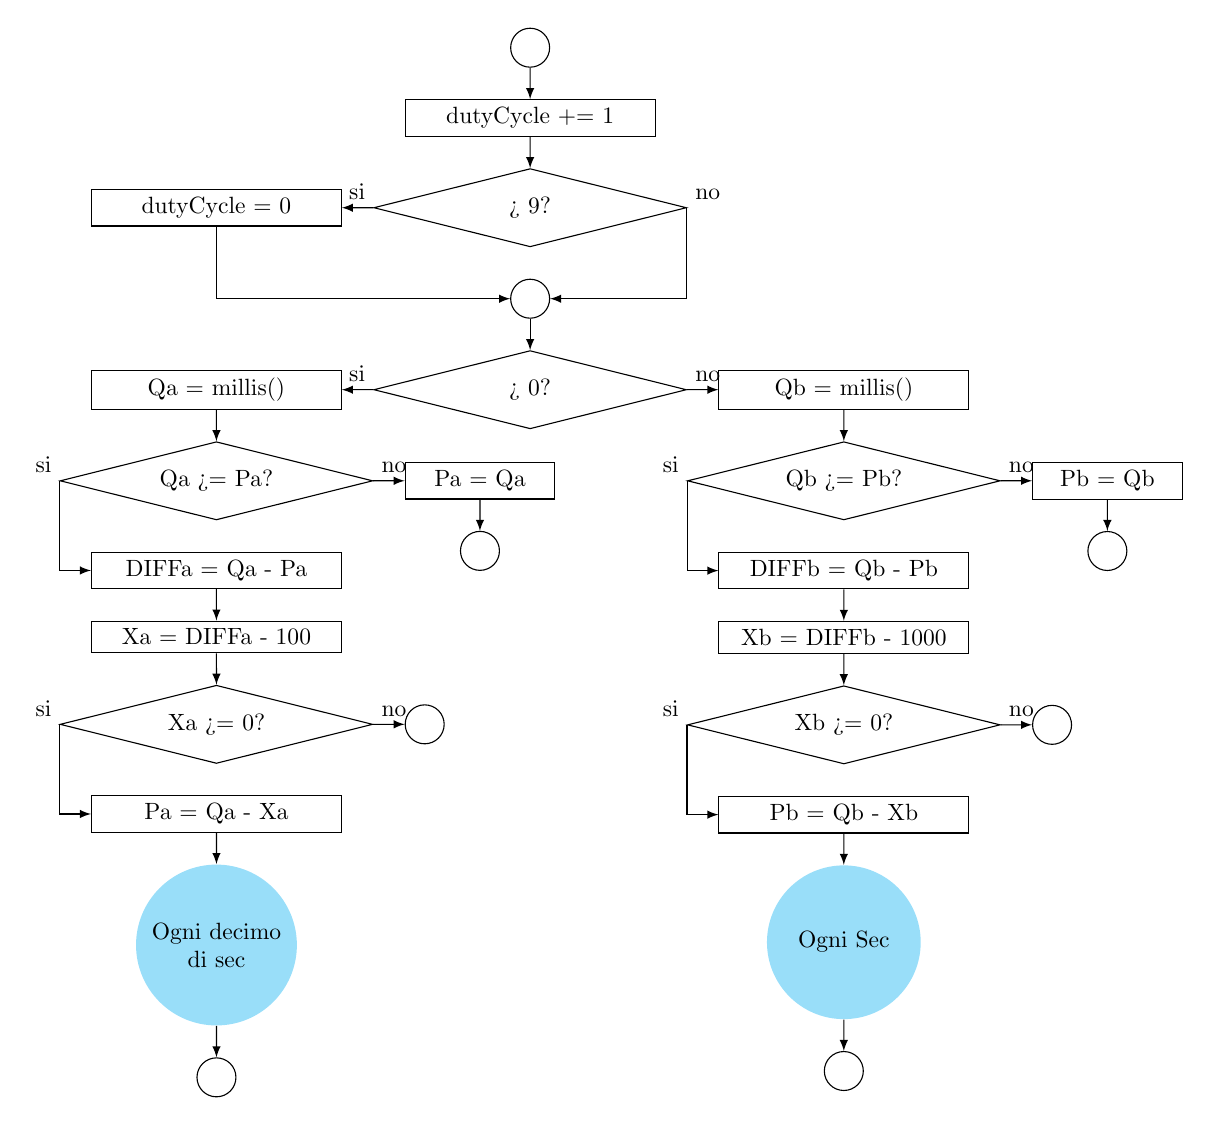
\begin{tikzpicture}[align=center,minimum height=3mm,node distance=4mm,scale=0.85, every node/.style={scale=0.85},
affermativo/.style={anchor=south east},
negativo/.style={anchor=south west},
testo/.style={draw,text width=3.5cm,anchor=north},
testoC/.style={text width=3.5cm,anchor=center},
condiz/.style={draw,diamond,aspect=4,text width=3.5cm},
cerchio/.style={draw,circle,text width=0.3cm}
]
\node[cerchio](xa){}; 	
%--
\node[testo,below=of xa](t){dutyCycle += 1};
\draw [-latex] (xa) -- (t);		
\node[condiz,below = of t,anchor=north](a){}; \node[testoC] at (a.center){> 9?};
\draw [-latex] (t) -- (a);		
\node[affermativo] (si) at (a.west){si};
\node[negativo] (no) at (a.east){no};
%--
\node[cerchio,below = of a,anchor=north ](xa){}; 	
\draw [-latex] (a.east) |- (xa);		
%--
\node[testo,left=of a](t){dutyCycle = 0};
\draw [-latex] (a.west) -- (t);		
\draw [-latex] (t) |- (xa);		
%--
\node[condiz,below = of xa,anchor=north](aaa){}; \node[testoC] at (aaa.center){> 0?};
\draw [-latex] (xa) -- (aaa);		
\node[affermativo] (si) at (aaa.west){si};
\node[negativo] (no) at (aaa.east){no};
%/////////////////////////////////////////////////////////
\node[testo,left=of aaa](t){Qa = millis()};
\draw [-latex] (aaa) -- (t);		
%--
\node[condiz,below = of t,anchor=north](a){}; \node[testoC] at (a.center){Qa >= Pa?};
\draw [-latex] (t) -- (a);		
\node[affermativo] (si) at (a.west){si};
\node[negativo] (no) at (a.east){no};
%--
\node[testo,text width=2cm,right=of a](t){Pa = Qa};
\draw [-latex] (a) -- (t);		
%--
\node[cerchio,below = of t,anchor=north ](xa){}; 	
\draw [-latex] (t) -- (xa);		
%----
\node[testo,below=of a](t){DIFFa = Qa - Pa}; %->>
\draw [-latex] (a.west) |- (t);		
%--
\node[testo,below=of t](a){Xa = DIFFa - 100};
\draw [-latex] (t) -- (a);		
%--
\node[condiz,below = of a,anchor=north](b){}; \node[testoC] at (b.center){Xa >= 0?};
\draw [-latex] (a) -- (b);		
\node[affermativo] (si) at (b.west){si};
\node[negativo] (no) at (b.east){no};
%--
\node[cerchio,right = of b](xa){}; 	
\draw [-latex] (b) -- (xa);		
%----
\node[testo,below=of b](t){Pa = Qa - Xa};
\draw [-latex] (b.west) |- (t);		
%----
\node[circle,text width=2cm,below=of t,fill=cyan!40](b){Ogni decimo di sec};
\draw [-latex] (t) -- (b);		
%--
\node[cerchio,below = of b](xa){}; 	
\draw [-latex] (b) -- (xa);		
%/////////////////////////////////////////////////////////
\node[testo,right=of aaa](t){Qb = millis()};
\draw [-latex] (aaa) -- (t);		
%--
\node[condiz,below = of t,anchor=north](a){}; \node[testoC] at (a.center){Qb >= Pb?};
\draw [-latex] (t) -- (a);		
\node[affermativo] (si) at (a.west){si};
\node[negativo] (no) at (a.east){no};
%--
\node[testo,text width=2cm,right=of a](t){Pb = Qb};
\draw [-latex] (a) -- (t);		
%--
\node[cerchio,below = of t,anchor=north ](xa){}; 	
\draw [-latex] (t) -- (xa);		
%----
\node[testo,below=of a](t){DIFFb = Qb - Pb}; %->>
\draw [-latex] (a.west) |- (t);		
%--
\node[testo,below=of t](a){Xb = DIFFb - 1000};
\draw [-latex] (t) -- (a);		
%--
\node[condiz,below = of a,anchor=north](b){}; \node[testoC] at (b.center){Xb >= 0?};
\draw [-latex] (a) -- (b);		
\node[affermativo] (si) at (b.west){si};
\node[negativo] (no) at (b.east){no};
%--
\node[cerchio,right = of b](xa){}; 	
\draw [-latex] (b) -- (xa);		
%----
\node[testo,below=of b](t){Pb = Qb - Xb};
\draw [-latex] (b.west) |- (t);		
%----
\node[circle,text width=2cm,below=of t,fill=cyan!40](b){Ogni Sec};
\draw [-latex] (t) -- (b);		
%--
\node[cerchio,below = of b](xa){}; 	
\draw [-latex] (b) -- (xa);		
\end{tikzpicture}
}
    \end{center}    
	\subsection{chkTEMPO}
    \begin{center}
        {\scriptsize
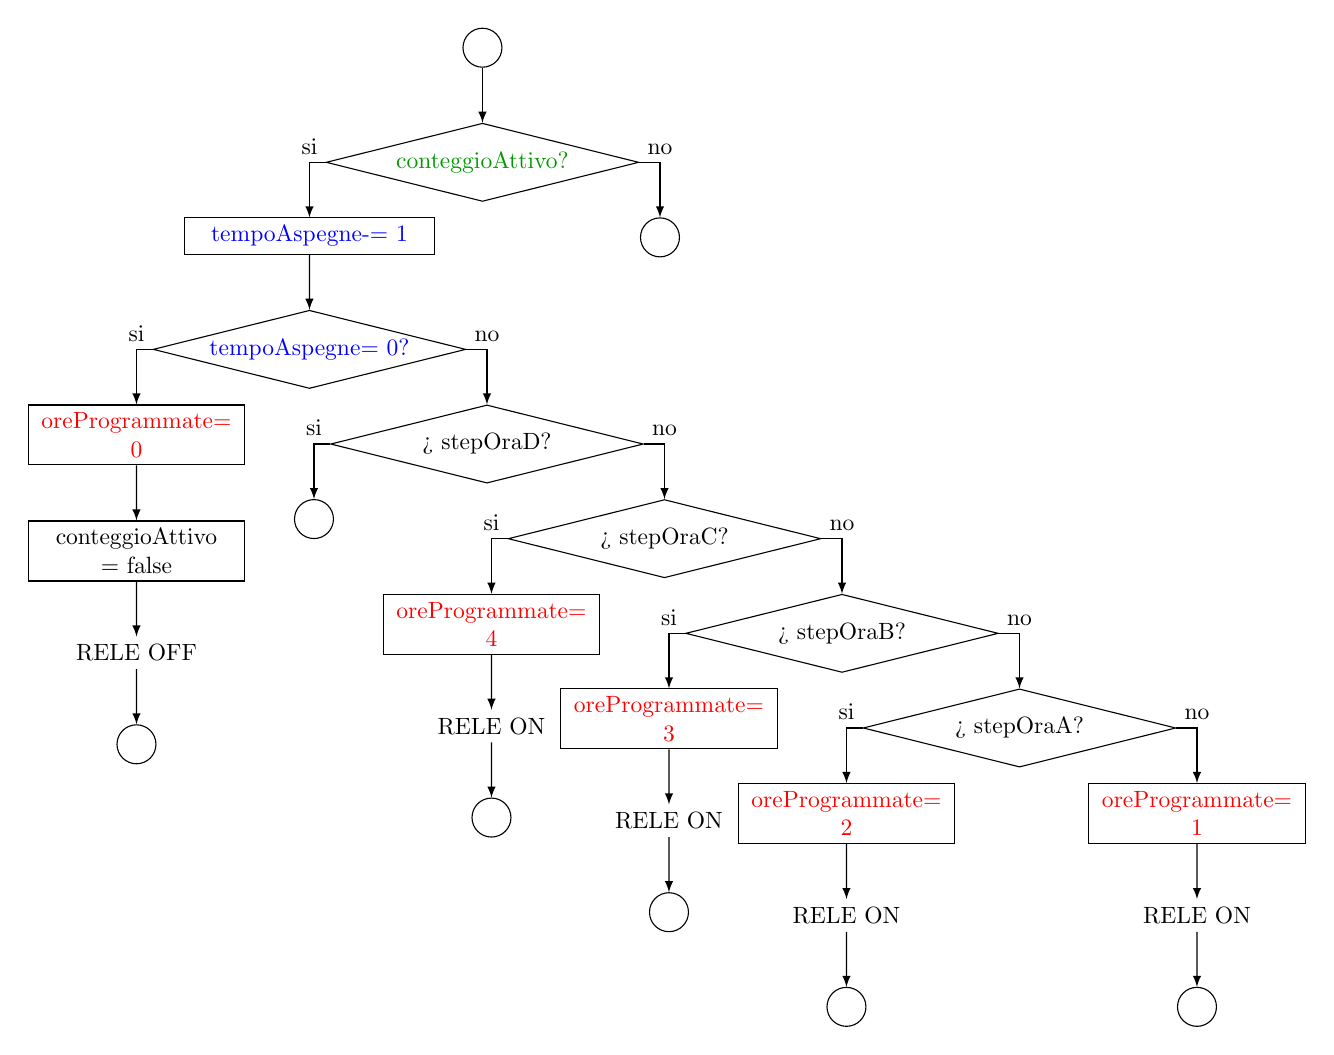
\begin{tikzpicture}[align=center,minimum height=3mm,node distance=7mm,scale=0.85, every node/.style={scale=0.85},
affermativo/.style={anchor=south east},
negativo/.style={anchor=south west},
testo/.style={draw,text width=3cm,anchor=north},
testoC/.style={text width=3.5cm,anchor=center},
condiz/.style={draw,diamond,aspect=4,text width=3.5cm},
cerchio/.style={draw,circle,text width=0.3cm}
]
\node[cerchio](xa){}; 	
%--
\node[condiz,below = of xa,anchor=north](a){}; \node[testoC] at (a.center){\conteggioAttivo?};
\draw [-latex] (xa) -- (a);		
\node[affermativo] (si) at (a.west){si};
\node[negativo] (no) at (a.east){no};
%--
\node[cerchio,below = of no,anchor=north ](xa){}; 	
\draw [-latex] (a.east) -| (xa);		
%--
\node[testo,text width=3.5cm,below = of si](b){\tempoAspegnimento -= 1};	
\draw [-latex] (a) -| (b);
%--
\node[condiz,below = of b,](bb){}; \node[testoC] at (bb.center){\tempoAspegnimento = 0?};
\node[affermativo] (si) at (bb.west){si};
\node[negativo] (no) at (bb.east){no};	
\draw [-latex] (b) -- (bb);
%--
\node[testo,below = of si](a){\oreProgrammate = 0};	
\draw [-latex] (bb) -| (a);	
\node[testo,below = of a](b){conteggioAttivo = false};	
\draw [-latex] (a) -- (b);	
\node[below = of b](a){RELE OFF};	
\draw [-latex] (b) -- (a);	
%--
\node[cerchio,below = of a,anchor=north ](xa){}; 
\draw [-latex] (a) -- (xa);		
%--		
\node[condiz,below = of no](aa){}; \node[testoC] at (aa.center){> stepOraD?};
\node[affermativo] (si) at (aa.west){si};
\node[negativo] (no) at (aa.east){no};	
\draw [-latex] (bb.east) -| (aa);
%--
\node[cerchio,below = of si](xa){}; 
\draw [-latex] (aa) -| (xa);	
%--		
\node[condiz,below = of no](a){}; \node[testoC] at (a.center){> stepOraC?};
\node[affermativo] (si) at (a.west){si};
\node[negativo] (no) at (a.east){no};	
\draw [-latex] (aa.east) -| (a);		
%--
\node[testo,below = of si](b){\oreProgrammate = 4};	
\draw [-latex] (a) -| (b);		
\node[below = of b](c){RELE ON};		
\draw [-latex] (b) -- (c);	
%--
\node[cerchio,below = of c,anchor=north ](xa){}; 
\draw [-latex] (c) -- (xa);		
%--		
\node[condiz,below = of no](b){}; \node[testoC] at (b.center){> stepOraB?};
\node[affermativo] (si) at (b.west){si};
\node[negativo] (no) at (b.east){no};	
\draw [-latex] (a.east) -| (b);
%--
\node[testo,below = of si](a){\oreProgrammate = 3};	
\draw [-latex] (b) -| (a);		
\node[below = of a](c){RELE ON};		
\draw [-latex] (a) -- (c);		
%--
\node[cerchio,below = of c,anchor=north ](xa){}; 
\draw [-latex] (c) -- (xa);		
%--		
\node[condiz,below = of no](aa){}; \node[testoC] at (aa.center){> stepOraA?};
\node[affermativo] (si) at (aa.west){si};
\node[negativo] (no) at (aa.east){no};	
\draw [-latex] (b.east) -| (aa);
%--
\node[testo,below = of si](b){\oreProgrammate = 2};	
\draw [-latex] (aa) -| (b);		
\node[below = of b](c){RELE ON};		
\draw [-latex] (b) -- (c);		
%--
\node[cerchio,below = of c,anchor=north ](xa){}; 
\draw [-latex] (c) -- (xa);	
%--
\node[testo,below =  of no](a){\oreProgrammate = 1};	
\draw [-latex] (aa) -| (a);		
\node[below = of a](c){RELE ON};		
\draw [-latex] (a) -- (c);		
%--
\node[cerchio,below = of c,anchor=north ](xa){}; 
\draw [-latex] (c) -- (xa);	
\end{tikzpicture}
}
    \end{center}
    \subsection{setLEDs}
    \begin{center}
        {\scriptsize
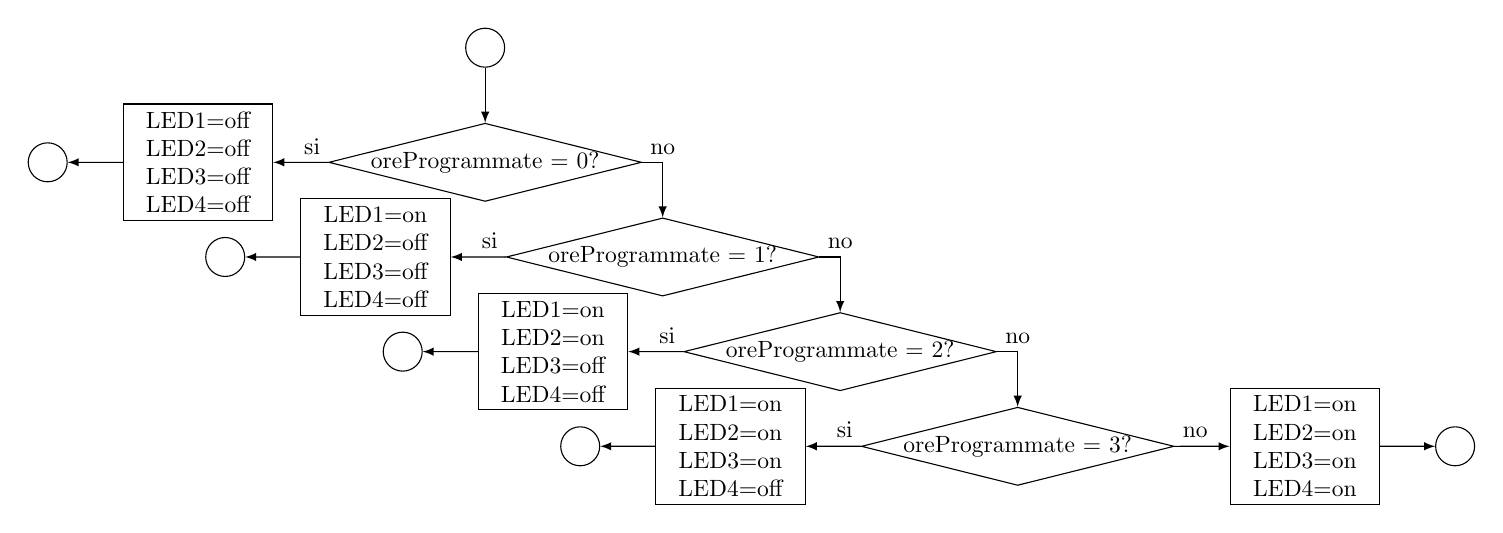
\begin{tikzpicture}[align=center,minimum height=3mm,node distance=7mm,scale=0.85, every node/.style={scale=0.85},
affermativo/.style={anchor=south east},
negativo/.style={anchor=south west},
testo/.style={draw,text width=2cm,anchor=north},
testoC/.style={text width=3.5cm,anchor=center},
condiz/.style={draw,diamond,aspect=4,text width=3.5cm},
cerchio/.style={draw,circle,text width=0.3cm}
]
\node[cerchio](xa){}; 	
%--
\node[condiz,below = of xa,anchor=north](a){}; \node[testoC] at (a.center){oreProgrammate = 0?};
\draw [-latex] (xa) -- (a);		
\node[affermativo] (si) at (a.west){si};
\node[negativo] (no) at (a.east){no};
%--
\node[testo,left=of a](t){LED1=off\\LED2=off\\LED3=off\\LED4=off};
\draw [-latex] (a) -- (t);		
\node[cerchio,left=of t](xa){};
\draw [-latex] (t) -- (xa);		
%----
\node[condiz,below = of no,anchor=north](b){}; \node[testoC] at (b.center){oreProgrammate = 1?};
\draw [-latex] (a) -| (b);		
\node[affermativo] (si) at (b.west){si};
\node[negativo] (no) at (b.east){no};
%--
\node[testo,left=of b](t){LED1=on\\LED2=off\\LED3=off\\LED4=off};
\draw [-latex] (b) -- (t);		
\node[cerchio,left=of t](xa){};
\draw [-latex] (t) -- (xa);		
%----
\node[condiz,below = of no,anchor=north](a){}; \node[testoC] at (a.center){oreProgrammate = 2?};
\draw [-latex] (b) -| (a);		
\node[affermativo] (si) at (a.west){si};
\node[negativo] (no) at (a.east){no};
%--
\node[testo,left=of a](t){LED1=on\\LED2=on\\LED3=off\\LED4=off};
\draw [-latex] (a) -- (t);		
\node[cerchio,left=of t](xa){};
\draw [-latex] (t) -- (xa);	
%----
\node[condiz,below = of no,anchor=north](b){}; \node[testoC] at (b.center){oreProgrammate = 3?};
\draw [-latex] (a) -| (b);		
\node[affermativo] (si) at (b.west){si};
\node[negativo] (no) at (b.east){no};
%--
\node[testo,left=of b](t){LED1=on\\LED2=on\\LED3=on\\LED4=off};
\draw [-latex] (b) -- (t);		
\node[cerchio,left=of t](xa){};
\draw [-latex] (t) -- (xa);	
%--
\node[testo,right=of b](t){LED1=on\\LED2=on\\LED3=on\\LED4=on};
\draw [-latex] (b.east) -- (t);		
\node[cerchio,right=of t](xa){};
\draw [-latex] (t) -- (xa);	 
\end{tikzpicture}}
    \end{center}       
    \subsection{chkPremuto}
    \begin{center}
        {\scriptsize
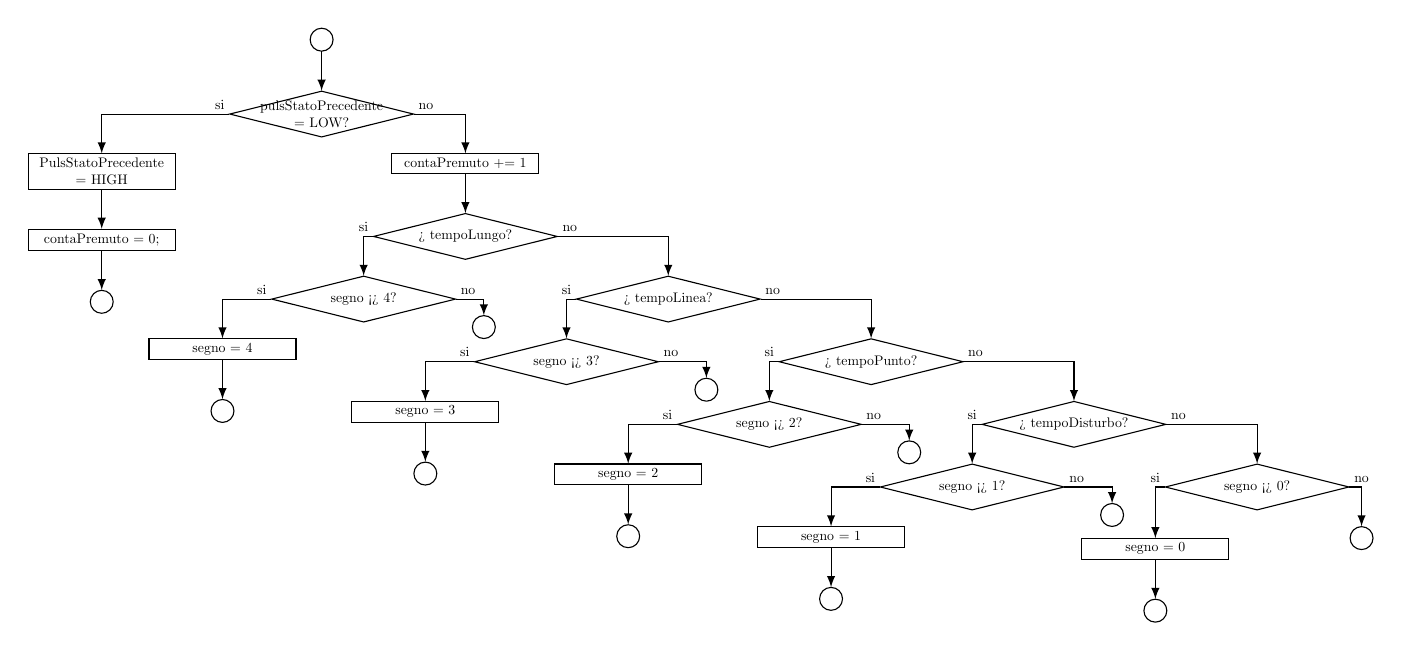
\begin{tikzpicture}[align=center,minimum height=3mm,node distance=5mm,scale=0.5, every node/.style={scale=0.5},
affermativo/.style={anchor=south east},
negativo/.style={anchor=south west},
testo/.style={draw,text width=3.5cm,anchor=north},
testoC/.style={text width=3.5cm,anchor=center},
condiz/.style={draw,diamond,aspect=4,text width=3.5cm},
cerchio/.style={draw,circle,text width=0.3cm}
]
\node[cerchio](xa){}; 	
%--
\node[condiz,below = of xa,anchor=north](a){}; \node[testoC] at (a.center){pulsStatoPrecedente = LOW?};
\draw [-latex] (xa) -- (a);		
\node[affermativo] (si) at (a.west){si};
\node[negativo] (no) at (a.east){no};
%--
\node[testo,below = of si,xshift=-3cm](b){PulsStatoPrecedente = HIGH};
\draw [-latex] (a.west) -| (b);	
\node[testo,below = of b](aa){contaPremuto = 0;};
\draw [-latex] (b) -- (aa);		
%\node[testo,below = of aa](b){segno = 0};
%\draw [-latex] (aa) -- (b);				
%--	
\node[cerchio,below = of aa,anchor=north ](xa){}; 	
\draw [-latex] (aa) -- (xa);		
%----
\node[testo,below = of no,xshift=1cm](b){contaPremuto += 1};	
\draw [-latex] (a.east) -| (b);		
%----
\node[condiz,below = of b](aaa){}; \node[testoC] at (aaa.center){> tempoLungo?}; %->>
\node[affermativo] (si) at (aaa.west){si};
\node[negativo] (noA) at (aaa.east){no};	
\draw [-latex] (b) -- (aaa);		
%--
\node[condiz,below = of si](bb){}; \node[testoC] at (bb.center){segno <> 4?};
\node[affermativo] (si) at (bb.west){si};
\node[negativo] (no) at (bb.east){no};	
\draw [-latex] (aaa) -| (bb);
%--
\node[testo,below = of si,xshift=-1cm](b){segno = 4};
\draw [-latex] (bb.west) -| (b);	
%--	
\node[cerchio, below = of b,anchor=north ](xa){}; 	
\draw [-latex] (b) -- (xa);					
%--	
\node[cerchio, right = of bb,anchor=north west,yshift=-0.5cm,xshift=-0.5cm](xa){}; 	
\draw [-latex] (bb) -| (xa);				
%----
\node[condiz,below = of noA,xshift=2.5cm](aaB){}; \node[testoC] at (aaB.center){> tempoLinea?}; %->>
\node[affermativo] (si) at (aaB.west){si};
\node[negativo] (noB) at (aaB.east){no};	
\draw [-latex] (aaa) -| (aaB);		
%--
\node[condiz,below = of si](bb){}; \node[testoC] at (bb.center){segno <> 3?};
\node[affermativo] (si) at (bb.west){si};
\node[negativo] (no) at (bb.east){no};	
\draw [-latex] (aaB) -| (bb);
%--
\node[testo,below = of si,xshift=-1cm](b){segno = 3};
\draw [-latex] (bb.west) -| (b);	
%--	
\node[cerchio, below = of b,anchor=north ](xa){}; 	
\draw [-latex] (b) -- (xa);					
%--	
\node[cerchio, right = of bb,anchor=north west,yshift=-0.5cm](xa){}; 	
\draw [-latex] (bb) -| (xa);	
%----
\node[condiz,below = of noB,xshift=2.5cm](aaC){}; \node[testoC] at (aaC.center){> tempoPunto?}; %->>
\node[affermativo] (si) at (aaC.west){si};
\node[negativo] (noC) at (aaC.east){no};	
\draw [-latex] (aaB) -| (aaC);		
%--
\node[condiz,below = of si](bb){}; \node[testoC] at (bb.center){segno <> 2?};
\node[affermativo] (si) at (bb.west){si};
\node[negativo] (no) at (bb.east){no};	
\draw [-latex] (aaC) -| (bb);
%--
\node[testo,below = of si,xshift=-1cm](b){segno = 2};
\draw [-latex] (bb.west) -| (b);	
%--	
\node[cerchio, below = of b,anchor=north ](xa){}; 	
\draw [-latex] (b) -- (xa);					
%--	
\node[cerchio, right = of bb,anchor=north west,yshift=-0.5cm](xa){}; 	
\draw [-latex] (bb) -| (xa);		
%----
\node[condiz,below = of noC,xshift=2.5cm](aaD){}; \node[testoC] at (aaD.center){> tempoDisturbo?}; %->>
\node[affermativo] (si) at (aaD.west){si};
\node[negativo] (noD) at (aaD.east){no};	
\draw [-latex] (aaC) -| (aaD);		
%--
\node[condiz,below = of si](bb){}; \node[testoC] at (bb.center){segno <> 1?};
\node[affermativo] (si) at (bb.west){si};
\node[negativo] (no) at (bb.east){no};	
\draw [-latex] (aaD) -| (bb);
%%--
\node[testo,below = of si,xshift=-1cm](b){segno = 1};
\draw [-latex] (bb.west) -| (b);	
%%--	
\node[cerchio, below = of b,anchor=north ](xa){}; 	
\draw [-latex] (b) -- (xa);					
%%--	
\node[cerchio, right = of bb,anchor=north west,yshift=-0.5cm](xa){}; 	
\draw [-latex] (bb) -| (xa);	
%--
\node[condiz,below = of noD,xshift=2cm](bb){}; \node[testoC] at (bb.center){segno <> 0?};
\node[affermativo] (si) at (bb.west){si};
\node[negativo] (no) at (bb.east){no};	
\draw [-latex] (aaD) -| (bb);
%%--
\node[testo,below = of si,yshift=-3mm](b){segno = 0};
\draw [-latex] (bb) -| (b);	
%--
\node[cerchio, below = of b,anchor=north ](xa){}; 	
\draw [-latex] (b) -- (xa);					
%--
\node[cerchio, below = of no,anchor=north ](xa){}; 	
\draw [-latex] (bb) -| (xa);					
\end{tikzpicture}
}
    \end{center}    
    \subsection{chkRilasciato}
    \begin{center}
        {\scriptsize
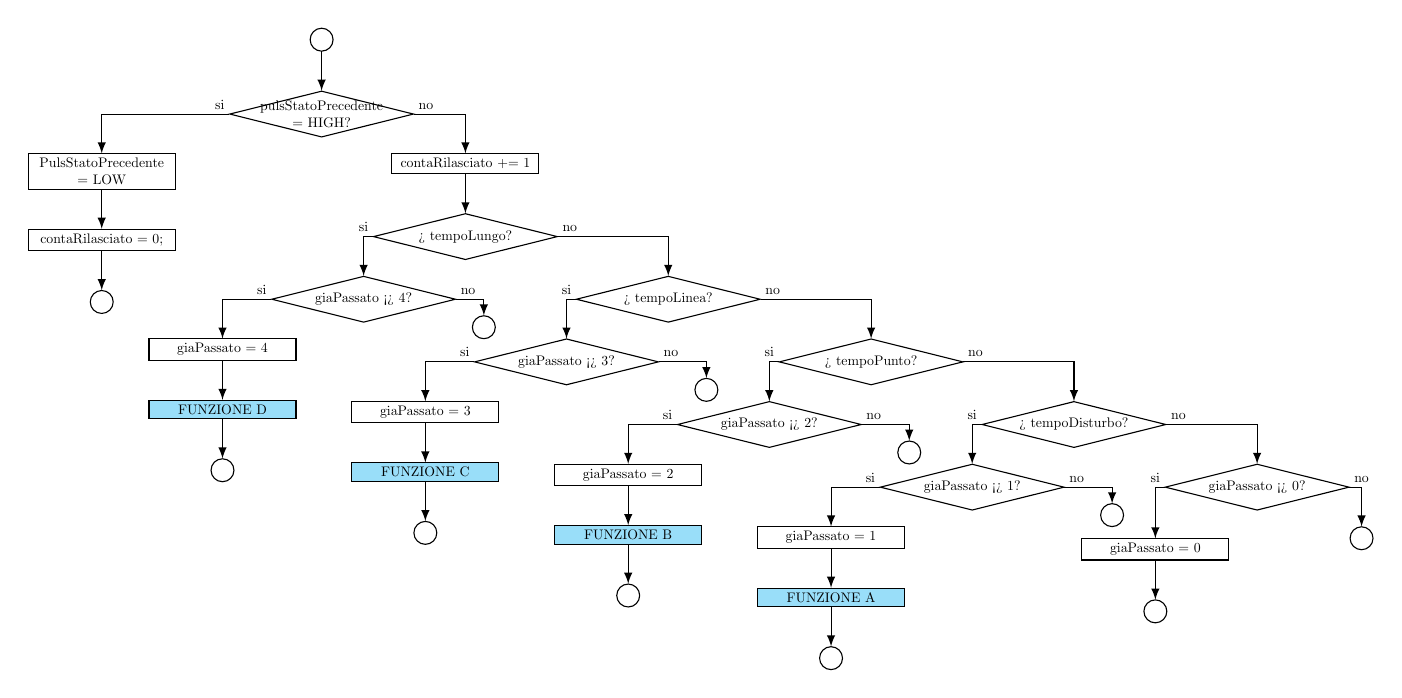
\begin{tikzpicture}[align=center,minimum height=3mm,node distance=5mm,scale=0.5, every node/.style={scale=0.5},
affermativo/.style={anchor=south east},
negativo/.style={anchor=south west},
testo/.style={draw,text width=3.5cm,anchor=north},
testoC/.style={text width=3.5cm,anchor=center},
condiz/.style={draw,diamond,aspect=4,text width=3.5cm},
cerchio/.style={draw,circle,text width=0.3cm}
]
\node[cerchio](xa){}; 	
%--
\node[condiz,below = of xa,anchor=north](a){}; \node[testoC] at (a.center){pulsStatoPrecedente = HIGH?};
\draw [-latex] (xa) -- (a);		
\node[affermativo] (si) at (a.west){si};
\node[negativo] (no) at (a.east){no};
%--
\node[testo,below = of si,xshift=-3cm](b){PulsStatoPrecedente = LOW};
\draw [-latex] (a.west) -| (b);	
\node[testo,below = of b](aa){contaRilasciato = 0;};
\draw [-latex] (b) -- (aa);		
%\node[testo,below = of aa](b){segno = 0};
%\draw [-latex] (aa) -- (b);				
%--	
\node[cerchio,below = of aa,anchor=north ](xa){}; 	
\draw [-latex] (aa) -- (xa);		
%----
\node[testo,below = of no,xshift=1cm](b){contaRilasciato += 1};	
\draw [-latex] (a.east) -| (b);		
%----
\node[condiz,below = of b](aaa){}; \node[testoC] at (aaa.center){> tempoLungo?}; %->>
\node[affermativo] (si) at (aaa.west){si};
\node[negativo] (noA) at (aaa.east){no};	
\draw [-latex] (b) -- (aaa);		
%--
\node[condiz,below = of si](bb){}; \node[testoC] at (bb.center){giaPassato <> 4?};
\node[affermativo] (si) at (bb.west){si};
\node[negativo] (no) at (bb.east){no};	
\draw [-latex] (aaa) -| (bb);
%--
\node[testo,below = of si,xshift=-1cm](b){giaPassato = 4};
\draw [-latex] (bb.west) -| (b);	
%--
\node[testo,below = of b,fill=cyan!40](a){FUNZIONE D};
\draw [-latex] (b) -- (a);		
%--	
\node[cerchio, below = of a,anchor=north ](xa){}; 	
\draw [-latex] (a) -- (xa);					
%--	
\node[cerchio, right = of bb,anchor=north west,yshift=-0.5cm,xshift=-0.5cm](xa){}; 	
\draw [-latex] (bb) -| (xa);				
%----
\node[condiz,below = of noA,xshift=2.5cm](aaB){}; \node[testoC] at (aaB.center){> tempoLinea?}; %->>
\node[affermativo] (si) at (aaB.west){si};
\node[negativo] (noB) at (aaB.east){no};	
\draw [-latex] (aaa) -| (aaB);		
%--
\node[condiz,below = of si](bb){}; \node[testoC] at (bb.center){giaPassato <> 3?};
\node[affermativo] (si) at (bb.west){si};
\node[negativo] (no) at (bb.east){no};	
\draw [-latex] (aaB) -| (bb);
%--
\node[testo,below = of si,xshift=-1cm](b){giaPassato = 3};
\draw [-latex] (bb.west) -| (b);	
%--
\node[testo,below = of b,fill=cyan!40](a){FUNZIONE C};
\draw [-latex] (b) -- (a);		
%--	
\node[cerchio, below = of a,anchor=north ](xa){}; 	
\draw [-latex] (a) -- (xa);					
%--	
\node[cerchio, right = of bb,anchor=north west,yshift=-0.5cm](xa){}; 	
\draw [-latex] (bb) -| (xa);	
%----
\node[condiz,below = of noB,xshift=2.5cm](aaC){}; \node[testoC] at (aaC.center){> tempoPunto?}; %->>
\node[affermativo] (si) at (aaC.west){si};
\node[negativo] (noC) at (aaC.east){no};	
\draw [-latex] (aaB) -| (aaC);		
%--
\node[condiz,below = of si](bb){}; \node[testoC] at (bb.center){giaPassato <> 2?};
\node[affermativo] (si) at (bb.west){si};
\node[negativo] (no) at (bb.east){no};	
\draw [-latex] (aaC) -| (bb);
%--
\node[testo,below = of si,xshift=-1cm](b){giaPassato = 2};
\draw [-latex] (bb.west) -| (b);	
%--
\node[testo,below = of b,fill=cyan!40](a){FUNZIONE B};
\draw [-latex] (b) -- (a);		
%--	
\node[cerchio, below = of a,anchor=north ](xa){}; 	
\draw [-latex] (a) -- (xa);					
%--	
\node[cerchio, right = of bb,anchor=north west,yshift=-0.5cm](xa){}; 	
\draw [-latex] (bb) -| (xa);		
%----
\node[condiz,below = of noC,xshift=2.5cm](aaD){}; \node[testoC] at (aaD.center){> tempoDisturbo?}; %->>
\node[affermativo] (si) at (aaD.west){si};
\node[negativo] (noD) at (aaD.east){no};	
\draw [-latex] (aaC) -| (aaD);		
%--
\node[condiz,below = of si](bb){}; \node[testoC] at (bb.center){giaPassato <> 1?};
\node[affermativo] (si) at (bb.west){si};
\node[negativo] (no) at (bb.east){no};	
\draw [-latex] (aaD) -| (bb);
%%--
\node[testo,below = of si,xshift=-1cm](b){giaPassato = 1};
\draw [-latex] (bb.west) -| (b);	
%%--
\node[testo,below = of b,fill=cyan!40](a){FUNZIONE A};
\draw [-latex] (b) -- (a);		
%%--
%\node[testo,below = of a](b){segno = 0};
%\draw [-latex] (a) -- (b);		
%%--	
\node[cerchio, below = of a,anchor=north ](xa){}; 	
\draw [-latex] (a) -- (xa);					
%%--	
\node[cerchio, right = of bb,anchor=north west,yshift=-0.5cm](xa){}; 	
\draw [-latex] (bb) -| (xa);	
%%--	
%\node[testo,below = of noD,yshift=-2cm](b){giaPassato = 0};
%\draw [-latex] (aaD) -| (b);		
%%--
%\node[cerchio, below = of b,anchor=north ](xa){}; 	
%\draw [-latex] (b) -- (xa);		
%----
\node[condiz,below = of noD,xshift=2cm](bb){}; \node[testoC] at (bb.center){giaPassato <> 0?};
\node[affermativo] (si) at (bb.west){si};
\node[negativo] (no) at (bb.east){no};	
\draw [-latex] (aaD) -| (bb);
%%--
\node[testo,below = of si,yshift=-3mm](b){giaPassato = 0};
\draw [-latex] (bb) -| (b);	
%--
\node[cerchio, below = of b,anchor=north ](xa){}; 	
\draw [-latex] (b) -- (xa);					
%--
\node[cerchio, below = of no,anchor=north ](xa){}; 	
\draw [-latex] (bb) -| (xa);					
\end{tikzpicture}
}
    \end{center}
\end{document}
